\documentclass[UTF8,zihao=-4]{ctexart}

\usepackage[a4paper,margin=1.8cm]{geometry}
\usepackage{graphicx}
\usepackage{pdflscape}
\usepackage{amsmath,amssymb}
\usepackage{array,tabularx,longtable,multirow}
\usepackage{enumitem}
\usepackage{listings}
\usepackage{fancyhdr}
\usepackage{lastpage}
\usepackage{forest}
\usetikzlibrary{automata,positioning,arrows.meta}

\setCJKmainfont{Source Han Serif CN}
\setCJKsansfont{Source Han Sans CN}
\setCJKmonofont{Noto Sans Mono CJK SC}
\setmonofont{DejaVu Sans Mono}

\pagestyle{fancy}
\fancyhf{}
\cfoot{第 \thepage 页共 \pageref{LastPage} 页}
\renewcommand{\headrulewidth}{0pt}

\setlength{\parindent}{0pt}
\setlength{\parskip}{0.35em}
\renewcommand{\arraystretch}{1.2}
\newcolumntype{L}[1]{>{\raggedright\arraybackslash}p{#1}}
\setlist[enumerate]{leftmargin=2.2em,itemsep=0.35em,topsep=0.2em}

\lstset{
  basicstyle=\ttfamily\small,
  columns=fullflexible,
  keepspaces=true,
  showstringspaces=false,
  xleftmargin=1.5em
}

\newcommand{\eps}{\varepsilon}
\newcommand{\gto}{\rightarrow}
\newcommand{\kw}[1]{\texttt{#1}}
\newcommand{\set}[1]{\{#1\}}
\newcommand{\ans}[1]{\textbf{#1}}
\newcommand{\chapters}[1]{\par\noindent{\small\textbf{涉及章节：}#1}\par}
\newcommand{\tattr}[2]{\begin{tabular}{@{}c@{}}\ensuremath{#1}\\[-0.15em]\scriptsize #2\end{tabular}}

\begin{document}

\begin{center}
  {\Large\bfseries 形式语言与编译考试题参考答案}\\
  \vspace{0.3em}
  {\normalsize 对应 \kw{exam\_17.tex}}
\end{center}

\section*{1. 判断正误}
\chapters{综合题。Slides：\kw{第一章2026.pdf}、\kw{第二章DFA2026.pdf}、\kw{第三章RL2026.pdf}、\kw{第四章2026.pdf}、\kw{第五章2026.pdf}、\kw{第六章-2026.pdf}、\kw{第十一章2026.pdf}；笔记：\kw{知识点总结.md} 第 1、2、3、4、5、6、11 章。}

\begin{center}
\begin{tabular}{c|cccccccccc}
题号 & (1) & (2) & (3) & (4) & (5) & (6) & (7) & (8) & (9) & (10)\\
\hline
答案 & 对 & 对 & 对 & 错 & 错 & 对 & 错 & 对 & 对 & 对
\end{tabular}
\end{center}

逐题解析：
\begin{enumerate}[label=(\arabic*)]
  \item \textbf{章节定位：}Slides \kw{第一章2026.pdf}；笔记第 1 章“中心概念与编译过程/基本概念”。对。$\eps$ 是任意字母表 $\Sigma$ 上的符号串，因为 $\eps\in\Sigma^*$；但它通常不是字母表中的符号，即 $\eps\notin\{a,d\}$。
  \item \textbf{章节定位：}Slides \kw{第二章DFA2026.pdf}；笔记第 2 章“DFA 定义/扩展转移函数”。对。DFA 的扩展转移函数 $\hat{\delta}$ 描述“从某状态读完整个串后到达的状态”，从开始状态 $q_0$ 读完 $x$ 后就是 $\hat{\delta}(q_0,x)$。
  \item \textbf{章节定位：}Slides \kw{第三章RL2026.pdf}；笔记第 3 章“正则语言判定性质/泵引理”。对。若一个 $n$ 状态 DFA 接受无穷语言，则必有可泵循环，因此接受串长度可以超过 $n$；反过来说，若所有接受串长度都不超过 $n$，最多只有有限多个串。
  \item \textbf{章节定位：}Slides \kw{第三章RL2026.pdf}；笔记第 3 章“泵引理/证明非正则”。错。语言 $\{w\mid \#0(w)=\#1(w)\}$ 需要无界计数匹配，不是正则语言，可用泵引理或 Myhill-Nerode 思路证明。
  \item \textbf{章节定位：}Slides \kw{第五章2026.pdf}；笔记第 5 章“CFG 定义”。错。CFG 至少要有开始符号 $S$，且 $S$ 必须是变元，所以变元集合不可能为空。
  \item \textbf{章节定位：}Slides \kw{第五章2026.pdf}、\kw{第八章-2026new.pdf}；笔记第 5 章“短语、直接短语、句柄”和第 8 章“规范归约”。对。句柄是规范归约中下一步应归约的直接短语，因此它一定是直接短语。
  \item \textbf{章节定位：}Slides \kw{第六章-2026.pdf}；笔记第 6 章“FIRST/FOLLOW/SELECT/预测分析表”。错。若 $N\gto\alpha$ 且 $\alpha\Rightarrow^*\eps$，预测分析表项还可由 $FOLLOW(N)$ 填入，所以 $M[N,c]=N\gto\alpha$ 时不一定有 $c\in FIRST(\alpha)$。
  \item \textbf{章节定位：}Slides \kw{第十一章2026.pdf}；笔记第 11 章“活动树、栈帧、活动生命周期”。对。不允许递归调用时，同一过程的新活动必须在上一次活动结束后才可能再次出现，所以同一过程活动生命周期不会相交。
  \item \textbf{章节定位：}Slides \kw{第一章2026.pdf}；笔记第 1 章“编译器相关术语/编译过程”。对。源语言和目标语言可以相同，例如源到源翻译器、优化型编译器都可能把某语言翻译成同一种语言的另一份程序。
  \item \textbf{章节定位：}Slides \kw{第四章2026.pdf}；笔记第 4 章“词法记号设计/全体一种”。对。实数词法单元的具体值很多，用“全体一种”记号如 $(NUM,3.14)$ 或 $(FLOAT,3.14)$ 更合理，而不是每个实数字面量单独一种。
\end{enumerate}

\clearpage
\section*{2. 填空}
\chapters{综合填空。Slides：\kw{第一章2026.pdf}、\kw{第二章NFA2026.pdf}、\kw{第九章2026.pdf}、\kw{第十章2026.pdf}、\kw{第十一章2026.pdf}；笔记：第 1、2、9、10、11 章。}

\begin{center}
\begin{longtable}{c|L{0.24\textwidth}|L{0.58\textwidth}}
空号 & 答案 & 解析\\
\hline
(1) & $S\cdot S$，即语言 $SS$ &
\textbf{章节定位：}Slides \kw{第一章2026.pdf}、\kw{第三章RE2026.pdf}；笔记第 1 章“语言/符号串”和第 3 章“语言运算”。\par
$s$ 是语言 $S$ 中的句子，表示 $s\in S$。串 $s\cdot s$ 是两个 $S$ 中句子的连接，所以属于连接语言 $S S$。这里的点号表示串连接，不是乘法。\\
\hline
(2) & $\eps$ &
\textbf{章节定位：}Slides \kw{第二章NFA2026.pdf}；笔记第 2 章“NFA 定义/接受条件”。\par
NFA 接受空串的条件是开始状态经过零步或若干 $\eps$ 转移后可到达终态。题目说“开始状态不是结束状态”，并且没有额外说明可通过 $\eps$ 转移到终态；按本空常规考点，开始状态非终态时不接受 $\eps$。\\
\hline
(3) & $2$ &
\textbf{章节定位：}Slides \kw{第九章2026.pdf}；笔记第 9 章“声明语义分析/数组声明”。\par
\kw{int a[2]} 是一维数组声明，方括号中的 $2$ 是这一维的长度，所以维数为 $1$，维长为 $2$。\\
\hline
(4) & \kw{int} &
\textbf{章节定位：}Slides \kw{第九章2026.pdf}；笔记第 9 章“声明语义分析/类型表达式”。\par
数组元素类型来自声明前面的类型说明符 \kw{int}。因此 $a$ 是元素类型为 \kw{int}、维长为 $2$ 的数组。\\
\hline
(5) & 结点 $N$ 的子结点 &
\textbf{章节定位：}Slides \kw{第九章2026.pdf}；笔记第 9 章“综合属性与继承属性”。\par
综合属性是自底向上计算的属性。某结点 $N$ 的综合属性只依赖它的子结点属性；继承属性才可能依赖父结点或左兄弟属性。\\
\hline
(6) & \kw{fp} &
\textbf{章节定位：}Slides \kw{第十一章2026.pdf}；笔记第 11 章“栈帧/活动记录”。\par
访问当前过程活动记录中的单元时，基址通常取当前活动记录基址，即帧指针 \kw{fp}。题目问“$f$ 的活动记录中 $x$ 单元”，所以基址是 $f$ 当前活动记录的 \kw{fp}。\\
\hline
(7) & $0$ &
\textbf{章节定位：}Slides \kw{第十一章2026.pdf}；笔记第 11 章“参数传递/栈帧布局”。\par
题目特别注明“不含参数个数单元”。若参数区从第一个形参开始编号，则 $x$ 是第一个形参，偏移量为 $0$；$y$ 才是下一个形参单元。\\
\hline
(8) & \kw{x b c + a * -} &
\textbf{章节定位：}Slides \kw{第十章2026.pdf}；笔记第 10 章“逆波兰式、三地址码、四元式、AST”。\par
先算括号内 $b+c$，逆波兰为 \kw{b c +}；再乘 $a$，得到 \kw{b c + a *}；最后用 $x$ 减去该结果，得到 \kw{x b c + a * -}。\\
\hline
(9) &
\begin{tabular}[t]{@{}l@{}}
\kw{t1 = b + c}\\
\kw{t2 = t1 * a}\\
\kw{t3 = x - t2}
\end{tabular}
&
\textbf{章节定位：}Slides \kw{第十章2026.pdf}；笔记第 10 章“表达式翻译/QTAC 指令形式”。\par
三地址码每条语句最多包含一个运算符。按照表达式求值顺序，先为 $b+c$ 建临时变量 $t1$，再为 $(b+c)*a$ 建 $t2$，最后计算 $x-t2$。\\
\hline
(10) & 代码区 &
\textbf{章节定位：}Slides \kw{第十一章2026.pdf}；笔记第 11 章“内存映像”。\par
运行时存储空间通常分为代码区、静态/全局区、堆区、栈区等。程序指令本身存放在代码区；活动记录在栈区，动态对象在堆区。\\
\end{longtable}
\end{center}

\section*{3. 十六进制小整数的正则表达式}
\chapters{Slides：\kw{第三章RE2026.pdf}，也可联系 \kw{第四章2026.pdf} 的词法记号设计；笔记：第 3 章“正则表达式与正则语言”、第 4 章“词法分析”。}

若不允许两位数出现前导 $0$，可写为：
\[
(\eps\mid +\mid -)\bigl(\texttt{[0-9A-F]}\mid \texttt{[1-7][0-9A-F]}\bigr).
\]

若允许 \kw{0F} 这类两位写法，则可写为：
\[
(\eps\mid +\mid -)\bigl(\texttt{[0-9A-F]}\mid \texttt{[0-7][0-9A-F]}\bigr).
\]

其中最高位不能超过 $7$，因为 $127_{10}=7F_{16}$。

解析：十六进制小整数最多两位，符号可有可无，所以最外层是 $(\eps\mid+\mid-)$。绝对值小于等于 $7F$，因此一位数可为任意十六进制位；两位数的高位只能是 $1$ 到 $7$，低位可为任意十六进制位。若允许前导 $0$，两位数高位也可取 $0$。

\section*{4. 文法题}
\chapters{总知识点：上下文无关文法的化简、FIRST/FOLLOW、二义性。Slides：\kw{第五章2026.pdf}、\kw{第六章-2026.pdf}；笔记：第 5 章“CFG、推导、语法树、文法化简”和第 6 章“LL(1)、FIRST、FOLLOW、预测分析”。}

\subsection*{4.1 消除无用符号}
\chapters{Slides：\kw{第五章2026.pdf}；笔记：第 5 章“消除无用符号”。}

\[
S\gto Aa\mid\eps,\qquad A\gto Aa,\qquad B\gto Bc\mid d
\]

$A$ 无产出；删去含 $A$ 的产生式后，$B$ 虽有产出但从 $S$ 不可达。故结果为：
\[
S\gto\eps.
\]

\subsection*{4.2 消除 $\eps$-产生式}
\chapters{Slides：\kw{第五章2026.pdf}/\kw{第六章-2026.pdf} 的文法清理；笔记：第 5 章“消除 $\eps$ 产生式”。}

原文法中可空变元为 $S,B,C$。先得：
\[
\begin{aligned}
S&\gto ABC\mid AB\mid AC\mid A,\\
A&\gto Bb\mid b\mid a,\\
B&\gto Cb\mid b.
\end{aligned}
\]

为保留原语言中的空串，引入新开始符号 $S_0$：
\[
S_0\gto S\mid\eps.
\]

若进一步删去已经无产出的 $C$，可化为更干净的等价文法：
\[
\boxed{
\begin{aligned}
S_0&\gto S\mid\eps,\\
S&\gto AB\mid A,\\
A&\gto Bb\mid b\mid a,\\
B&\gto b.
\end{aligned}}
\]

\subsection*{4.3 消除单位产生式}
\chapters{Slides：\kw{第五章2026.pdf}/\kw{第六章-2026.pdf} 的文法清理；笔记：第 5 章“消除单位产生式”。}

单位产生式为 $E\gto T$、$T\gto F$，并且 $E\Rightarrow T\Rightarrow F$。把可达变元的非单位产生式补到左部，得到：
\[
\boxed{
\begin{aligned}
E&\gto E+T\mid T*F\mid i\mid(E),\\
T&\gto T*F\mid i\mid(E),\\
F&\gto i\mid(E).
\end{aligned}}
\]

\subsection*{4.4 消除左递归}
\chapters{Slides：\kw{第六章-2026.pdf}；笔记：第 5 章“消除左递归”和第 6 章“LL(1) 的含义/LL(1) 判定”。}

原文法：
\[
S\gto AB\mid a,\qquad A\gto Ab\mid Ba,\qquad B\gto Ac\mid d.
\]

按顺序处理 $A,B$。这个顺序下，处理 $A$ 时只消除已经显露出来的直接左递归；
$A\gto Ba$ 中的 $B$ 是后面的变元，暂不把 $B$ 代入 $A$。先消除 $A$ 的直接左递归：
\[
A\gto BaA',\qquad A'\gto bA'\mid\eps.
\]

再处理 $B$。此时 $B\gto Ac$ 的右部以已经处理过的 $A$ 开头，所以把 $A$ 的候选式代入：
\[
B\gto BaA'c\mid d.
\]

这样，原来 $B\Rightarrow Ac\Rightarrow Bac$ 的间接左递归被显露成了直接左递归
$B\gto BaA'c$。再消除 $B$ 的直接左递归：
\[
B\gto dB',\qquad B'\gto aA'cB'\mid\eps.
\]

最后把 $A\gto BaA'$ 中的 $B$ 用新的 $B\gto dB'$ 代入，得到一种无左递归文法：
\[
\boxed{
\begin{aligned}
S&\gto AB\mid a,\\
A&\gto dB'aA',\\
A'&\gto bA'\mid\eps,\\
B&\gto dB',\\
B'&\gto aA'cB'\mid\eps.
\end{aligned}}
\]

\subsection*{4.5 FIRST 与 FOLLOW}
\chapters{Slides：\kw{第六章-2026.pdf}；笔记：第 6 章“FIRST 集”“FOLLOW 集”。}

文法：
\[
S\gto P\mid o,\qquad P\gto i(B)SF,\qquad F\gto eS\mid\eps,\qquad B\gto 0\mid 1.
\]

\[
FIRST(S)=\{i,o\},\qquad FIRST(F)=\{e,\eps\}.
\]

开始符号 $S$ 的 FOLLOW 集含 $\#$。由 $P\gto i(B)SF$ 可知：
\[
FOLLOW(B)=\{)\}.
\]

又因为 $F$ 在 $P$ 的末尾，且 $S$ 后跟可空的 $F$，可得：
\[
FOLLOW(F)=FOLLOW(P)=FOLLOW(S)=\{\#,e\}.
\]

所以：
\[
\boxed{FOLLOW(F)=\{\#,e\},\qquad FOLLOW(B)=\{)\}.}
\]

\subsection*{4.6 二义性}
\chapters{Slides：\kw{第五章2026.pdf} 的“最左、最右推导”“语法树”“二义文法”“二义性与最左/最右推导”；笔记：第 5 章“推导、语法树”和“二义文法”。}

文法：
\[
E\gto E/E\mid E\&E\mid i.
\]

句子 $i/i\&i$ 有两个最左推导。

推导的找法：先观察句子中有两个运算符 $/$ 和 $\&$。文法没有规定优先级和结合性，因此最外层运算符可以先选 $/$，也可以先选 $\&$：
\[
i/i\&i
\quad\text{可以看作}\quad
i/(i\&i)
\quad\text{或}\quad
(i/i)\&i.
\]
这两个括号化方式对应两棵不同语法树。写最左推导时，每一步都只替换当前句型中最左边的变元 $E$。

推导一，对应结构 $i/(i\&i)$：
\[
E\Rightarrow E/E\Rightarrow i/E\Rightarrow i/E\&E
\Rightarrow i/i\&E\Rightarrow i/i\&i.
\]

推导二，对应结构 $(i/i)\&i$：
\[
E\Rightarrow E\&E\Rightarrow E/E\&E
\Rightarrow i/E\&E\Rightarrow i/i\&E\Rightarrow i/i\&i.
\]

对应语法树如下：

\begin{center}
\begin{minipage}{0.46\textwidth}
\centering
\textbf{结构 $i/(i\&i)$}

\begin{forest}
for tree={
  math content,
  parent anchor=south,
  child anchor=north,
  l sep=8mm,
  s sep=6mm,
  inner sep=1pt,
  align=center
}
[E
  [E
    [i]
  ]
  [/]
  [E
    [E
      [i]
    ]
    [\&]
    [E
      [i]
    ]
  ]
]
\end{forest}
\end{minipage}
\hfill
\begin{minipage}{0.46\textwidth}
\centering
\textbf{结构 $(i/i)\&i$}

\begin{forest}
for tree={
  math content,
  parent anchor=south,
  child anchor=north,
  l sep=8mm,
  s sep=6mm,
  inner sep=1pt,
  align=center
}
[E
  [E
    [E
      [i]
    ]
    [/]
    [E
      [i]
    ]
  ]
  [\&]
  [E
    [i]
  ]
]
\end{forest}
\end{minipage}
\end{center}

因此该文法是二义文法。

\section*{5. NFA 的 $\eps$-闭包与子集法}
\chapters{Slides：\kw{第二章NFA2026.pdf}；笔记：第 2 章“DFA、NFA、$\eps$-NFA”。}

\subsection*{5.1 原 NFA 状态图与 $\eps$-闭包}

由题目给出的 NFA 迁移表可读出如下状态图。状态 $1$ 是初态，状态 $5$ 是接受态。

\begin{center}
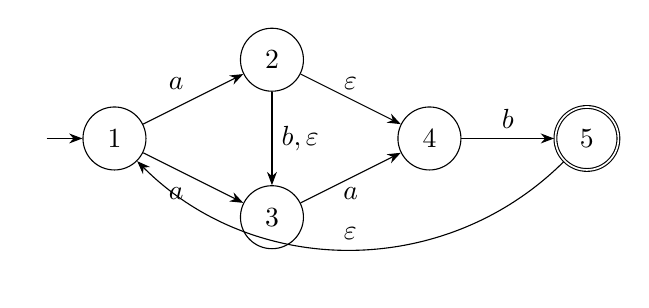
\begin{tikzpicture}[
  >=Stealth,
  node distance=20mm,
  every state/.style={minimum size=8mm},
  initial text={}
]
  \node[state, initial] (q1) at (0,0) {$1$};
  \node[state] (q2) at (2,1) {$2$};
  \node[state] (q3) at (2,-1) {$3$};
  \node[state] (q4) at (4,0) {$4$};
  \node[state, accepting] (q5) at (6,0) {$5$};

  \path[->]
    (q1) edge node[above left] {$a$} (q2)
    (q1) edge node[below left] {$a$} (q3)
    (q2) edge node[right] {$b,\eps$} (q3)
    (q2) edge node[above] {$\eps$} (q4)
    (q3) edge node[below] {$a$} (q4)
    (q4) edge node[above] {$b$} (q5)
    (q5) edge[bend left=45] node[above] {$\eps$} (q1);
\end{tikzpicture}
\end{center}

\[
\begin{aligned}
\eps\text{-closure}(1)&=\{1\},\\
\eps\text{-closure}(2)&=\{2,3,4\},\\
\eps\text{-closure}(3)&=\{3\},\\
\eps\text{-closure}(4)&=\{4\},\\
\eps\text{-closure}(5)&=\{5,1\}.
\end{aligned}
\]

\subsection*{5.2 转换为 DFA}

设初态：
\[
A=\{1\}.
\]

逐步求
\[
T=\eps\text{-closure}\left(\bigcup_{q\in S}\delta(q,x)\right),\qquad x\in\{a,b\}.
\]
若某一步得到 $\emptyset$，表示该输入下没有可达状态。本解答采用课件中常见的最简形 DFA 画法：$\emptyset$ 不单独命名为一个状态，画图时也不画通向死状态的边。

得到 DFA 迁移表：

\begin{center}
\begin{tabular}{c|c|c|c|c}
DFA 状态 & NFA 状态集合 & $a$ & $b$ & 是否接受\\
\hline
$A$ & $\{1\}$ & $B$ & $\emptyset$ & 否\\
$B$ & $\{2,3,4\}$ & $C$ & $D$ & 否\\
$C$ & $\{4\}$ & $\emptyset$ & $E$ & 否\\
$D$ & $\{1,3,5\}$ & $B$ & $\emptyset$ & 是\\
$E$ & $\{1,5\}$ & $B$ & $\emptyset$ & 是
\end{tabular}
\end{center}

其中接受态是包含原 NFA 接受态 $5$ 的集合，即 $D,E$。

由上表画出 DFA 状态图如下。图中没有画出 $\emptyset$ 对应的死状态，因此没有可达状态的转移边直接省略。

\begin{center}
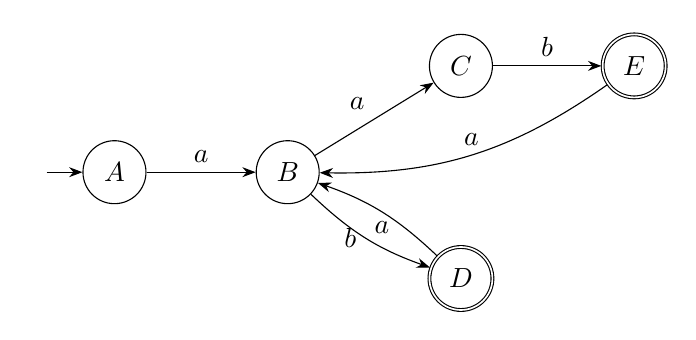
\begin{tikzpicture}[
  >=Stealth,
  node distance=22mm,
  every state/.style={minimum size=8mm},
  initial text={}
]
  \node[state, initial] (A) at (0,0) {$A$};
  \node[state] (B) at (2.2,0) {$B$};
  \node[state] (C) at (4.4,1.35) {$C$};
  \node[state, accepting] (D) at (4.4,-1.35) {$D$};
  \node[state, accepting] (E) at (6.6,1.35) {$E$};

  \path[->]
    (A) edge node[above] {$a$} (B)
    (B) edge node[above left] {$a$} (C)
    (B) edge[bend right=12] node[left] {$b$} (D)
    (C) edge node[above] {$b$} (E)
    (D) edge[bend right=12] node[below] {$a$} (B)
    (E) edge[bend left=18] node[above] {$a$} (B);
\end{tikzpicture}
\end{center}

若题目或老师要求“完全形 DFA”，则应额外加入死状态 $Z=\emptyset$，并把所有 $\emptyset$ 转移指向 $Z$。但按本题这种画图答法，不列 $Z$ 也是可以的。

\subsection*{5.3 DFA 最小化：划分法}

本小问还涉及 DFA 最小化，参考 Slides：\kw{第三章RL2026.pdf} 中的“DFA 最小化的划分算法”。这里沿用上面的最简形 DFA 约定：$\emptyset$ 只表示无转移，不作为状态参加划分。

先按是否接受划分：
\[
P_0=\bigl\{\{D,E\},\{A,B,C\}\bigr\}.
\]

考察每个状态在输入 $a,b$ 下转移到的划分块。用 $\bot$ 表示转移到 $\emptyset$，即无可达状态。相对于 $P_0$，有
\[
\begin{array}{c|c}
\text{状态} & (a,b)\text{ 到达的块}\\
\hline
A & (\{A,B,C\},\bot)\\
B & (\{A,B,C\},\{D,E\})\\
C & (\bot,\{D,E\})\\
D & (\{A,B,C\},\bot)\\
E & (\{A,B,C\},\bot)
\end{array}
\]
因此非接受态块 $\{A,B,C\}$ 分裂为 $\{A\}$、$\{B\}$、$\{C\}$，而接受态块 $\{D,E\}$ 暂不分裂，得到
\[
P_1=\bigl\{\{D,E\},\{A\},\{B\},\{C\}\bigr\}.
\]

继续相对于 $P_1$ 检查：
\[
\begin{array}{c|c}
\text{状态} & (a,b)\text{ 到达的块}\\
\hline
D & (\{B\},\bot)\\
E & (\{B\},\bot)
\end{array}
\]
所以 $\{D,E\}$ 不再分裂，最终划分为
\[
P_1=\bigl\{\{A\},\{B\},\{C\},\{D,E\}\bigr\}.
\]

因此只有 $D$ 与 $E$ 等价，可以合并。记
\[
X=\{D,E\}.
\]
最小 DFA 的迁移表为：

\begin{center}
\begin{tabular}{c|c|c|c}
最小 DFA 状态 & $a$ & $b$ & 是否接受\\
\hline
$A$ & $B$ & $\emptyset$ & 否\\
$B$ & $C$ & $X$ & 否\\
$C$ & $\emptyset$ & $X$ & 否\\
$X=\{D,E\}$ & $B$ & $\emptyset$ & 是
\end{tabular}
\end{center}

最小 DFA 状态图如下，同样省略 $\emptyset$ 死状态及其相关边。

\begin{center}
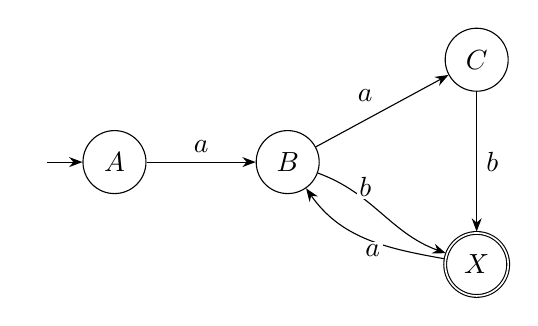
\begin{tikzpicture}[
  >=Stealth,
  node distance=22mm,
  every state/.style={minimum size=8mm},
  initial text={}
]
  \node[state, initial] (mA) at (0,0) {$A$};
  \node[state] (mB) at (2.2,0) {$B$};
  \node[state] (mC) at (4.6,1.3) {$C$};
  \node[state, accepting] (mX) at (4.6,-1.3) {$X$};

  \path[->]
    (mA) edge node[above] {$a$} (mB)
    (mB) edge node[above left] {$a$} (mC)
    (mB) edge[out=-20,in=160] node[pos=0.35, above, fill=white, inner sep=1pt] {$b$} (mX)
    (mC) edge node[right] {$b$} (mX)
    (mX) edge[out=170,in=-55] node[pos=0.45, below, fill=white, inner sep=1pt] {$a$} (mB);
\end{tikzpicture}
\end{center}

\section*{6. 活前缀 DFA 与冲突}
\chapters{Slides：\kw{第八章-2026new.pdf}；笔记：第 8 章“规范归约、LR(0)、SLR(1)”。}

增广文法：
\[
S'\gto S,\qquad S\gto E=n\mid +,\qquad E\gto n\mid n+.
\]

LR(0) 项目集为：
\[
\begin{aligned}
I_0=\{&S'\gto\cdot S,\ S\gto\cdot E=n,\ S\gto\cdot +,\ E\gto\cdot n,\ E\gto\cdot n+\},\\
I_1=\{&S'\gto S\cdot\},\\
I_2=\{&S\gto E\cdot =n\},\\
I_3=\{&S\gto +\cdot\},\\
I_4=\{&E\gto n\cdot,\ E\gto n\cdot +\},\\
I_5=\{&S\gto E=\cdot n\},\\
I_6=\{&S\gto E=n\cdot\},\\
I_7=\{&E\gto n+\cdot\}.
\end{aligned}
\]

下面的表是识别活前缀的 LR(0) itemDFA 转移表，也就是各项目集之间的
\(\mathrm{goto}\) 关系；它还不是 ACTION/GOTO 分析表。

\begin{center}
\begin{tabular}{c|ccccc}
状态 & $S$ & $E$ & $+$ & $n$ & $=$\\
\hline
$I_0$ & $I_1$ & $I_2$ & $I_3$ & $I_4$ & \\
$I_2$ & & & & & $I_5$\\
$I_4$ & & & $I_7$ & &\\
$I_5$ & & & & $I_6$ &
\end{tabular}
\end{center}

$I_4$ 中同时有归约项目 $E\gto n\cdot$ 和移进项目 $E\gto n\cdot+$，所以存在 LR(0) 移进-归约冲突。

用 SLR(1) 可消解该冲突。因为：
\[
FOLLOW(E)=\{=\}.
\]

故在输入 $=$ 时按 $E\gto n$ 归约；在输入 $+$ 时移进。这样冲突被 FOLLOW 集消解。

若进一步写成 SLR(1) 的 ACTION/GOTO 分析表，可按如下产生式编号：
\[
(1)\ S\gto E=n,\qquad (2)\ S\gto +,\qquad
(3)\ E\gto n,\qquad (4)\ E\gto n+.
\]

\begin{center}
\begin{tabular}{c|cccc|cc}
\multirow{2}{*}{状态} & \multicolumn{4}{c|}{ACTION} & \multicolumn{2}{c}{GOTO}\\
 & $n$ & $+$ & $=$ & $\#$ & $S$ & $E$\\
\hline
0 & s4 & s3 & & & 1 & 2\\
1 & & & & acc & &\\
2 & & & s5 & & &\\
3 & & & & r2 & &\\
4 & & s7 & r3 & & &\\
5 & s6 & & & & &\\
6 & & & & r1 & &\\
7 & & & r4 & & &
\end{tabular}
\end{center}

这里最关键的是状态 \(4\)：LR(0) 看见 \(E\gto n\cdot\) 会想在所有输入上归约，
同时又因为 \(E\gto n\cdot+\) 会在 \(+\) 上移进，所以有移进-归约冲突。
SLR(1) 用 \(FOLLOW(E)=\{=\}\) 限制归约，只在 \(=\) 上填 \(r3\)，而在 \(+\) 上填 \(s7\)，
因此表中没有冲突。

\section*{7. 运行时栈快照}
\chapters{Slides：\kw{第十一章2026.pdf}；笔记：第 11 章“运行时环境、栈帧、调用序列”。}

按题图中的栈快照格式，每个单元直接写成“单元名:值”。当前调用链为
\[
\kw{test}\to\kw{hool}\to\kw{bar(foo,x)}\to\kw{foo(x)}.
\]
控制链沿调用者回退；访问链沿词法外层回退。由于 \kw{foo}、\kw{bar}、\kw{hool} 都直接声明在 \kw{test} 内，所以它们的访问链均指向 \kw{test@frame}。

\begin{center}
\begin{longtable}{c|c|l}
活动记录 & 地址 & 栈单元内容\\
\hline
\multirow{3}{*}{\kw{test@frame}} &
100 & \kw{<访问链>}:$0$\\
& 099 & \kw{<控制链>}:$0$\\
& 098 & \kw{<返址>}:$0$\\
\hline
\multirow{4}{*}{\kw{hool@frame}} &
097 & \kw{<访问链>}:$100$\\
& 096 & \kw{<控制链>}:$100$\\
& 095 & \kw{<返址>}:$L_{\text{after-hool}}$\\
& 094 & \kw{x}:$3$\\
\hline
\multirow{7}{*}{\kw{bar@frame}} &
093 & \kw{x}:$094$\\
& 092 & \kw{t}:$087$\\
& 091 & \kw{<访问链>}:$100$\\
& 090 & \kw{<控制链>}:$097$\\
& 089 & \kw{<返址>}:$L_{\text{after-bar}}$\\
& 088 & \kw{t[1]}:$100$\\
& 087 & \kw{t[0]}:\kw{foo@label}\\
\hline
\multirow{4}{*}{\kw{foo@frame}} &
086 & \kw{y}:$094$\\
& 085 & \kw{<访问链>}:$100$\\
& 084 & \kw{<控制链>}:$093$\\
& 083 & \kw{<返址>}:$L_{\text{after-t-call}}$\\
\hline
\end{longtable}
\end{center}

因此：
\[
\boxed{fp=086,\qquad sp=083.}
\]

\kw{x}:$094$ 和 \kw{y}:$094$ 表示 \kw{var} 参数保存的是实参 \kw{hool.x} 的地址；\kw{t[0]} 是过程入口，\kw{t[1]} 是过程 \kw{foo} 携带的声明环境。若教材约定链指针指向控制链单元，则链值会相应换成各活动记录控制链单元地址；本表按题图 \kw{fp}/\kw{sp} 标法填写。

\section*{8. 属性文法与四元式}
\chapters{Slides：\kw{第九章2026.pdf}、\kw{第十章2026.pdf}；笔记：第 9 章“属性文法、符号表、声明语义分析”和第 10 章“QTAC、QAST、中间代码生成”。}

句子：
\[
\kw{if }x<>y\kw{ then while }x<y\lor x=a\kw{ do }y:=a+b.
\]

\subsection*{8.1 语法树}

按照题目给出的属性文法，句子对应的语法树如下。内结点框内标注规约后的关键属性值。注意题目说明中
$merge(p,q)$ 的返回链头是 $q$，所以这里用“链头 $\to$ 后继”的形式写链：例如
$E_3.tc=104\to102$，$S.chain=105\to101$。

\begin{landscape}
\begin{center}
\resizebox{!}{0.90\textheight}{%
\begin{forest}
for tree={
  parent anchor=south,
  child anchor=north,
  l sep=9mm,
  s sep=5mm,
  inner sep=2pt,
  font=\scriptsize,
  align=center,
  edge={-},
  if n children=0{draw=none, inner sep=1pt}{draw, rounded corners=2pt}
}
[{\tattr{S}{\(\mathrm{chain}=105\to101\)}}
  [{\tattr{C}{\(\mathrm{chain}=101\)}}
    [\texttt{if}]
    [{\tattr{E_0}{\(\mathrm{tc}=100,\ \mathrm{fc}=101\)}}
      [$x$][{$<>$}][$y$]
    ]
    [\texttt{then}]
  ]
  [{\tattr{S_1}{\(\mathrm{chain}=105\)}}
    [{\tattr{W^d}{\(\mathrm{quad}=102,\ \mathrm{chain}=105\)}}
      [{\tattr{W}{\(\mathrm{quad}=102\)}}
        [\texttt{while}]
      ]
      [{\tattr{E_3}{\(\mathrm{tc}=104\to102,\ \mathrm{fc}=105\)}}
        [{\tattr{E^\circ}{\(\mathrm{tc}=102\)}}
          [{\tattr{E_1}{\(\mathrm{tc}=102,\ \mathrm{fc}=103\)}}
            [$x$][{$<$}][$y$]
          ]
          [{$\lor$}]
        ]
        [{\tattr{E_2}{\(\mathrm{tc}=104,\ \mathrm{fc}=105\)}}
          [$x$][{$=$}][$a$]
        ]
      ]
      [\texttt{do}]
    ]
    [{\tattr{S_2}{\(\mathrm{chain}=0\)}}
      [$y$][{$:=$}][$a$][{$+$}][$b$]
    ]
  ]
]
\end{forest}%
}
\end{center}
\end{landscape}
\clearpage

\subsection*{8.2 属性逐步计算过程}

属性文法采用自底向上的方式，每应用一条产生式就立即执行对应的语义动作。下表按归约顺序排列，$nxq$ 列是\textbf{执行完该步后} $nxq$ 的值：

\begin{center}
\begin{longtable}{c|L{0.26\textwidth}|c|L{0.42\textwidth}}
步 & 归约产生式（当前句型中的子树） & $nxq$ & 语义动作与结果\\
\hline
1 & $E\gto i^2\,rop\,i^2$，匹配 $x<>y$ &
  102 &
  $Gen(j{<>},x,y,0)\Rightarrow\text{四元}100$（目标暂0）；$E_0.tc=100$。$Gen(j,\_,\_,0)\Rightarrow\text{四元}101$；$E_0.fc=101$。\\
\hline
2 & $C\gto \kw{if}\ E\ \kw{then}$，消费 $E_0$ &
  102 &
  $bp(E_0.tc{=}100,\ nxq{=}102)$：把四元 100 的目标填为 102。$C.chain=E_0.fc=101$（if 为假时的出口，留悬空）。\\
\hline
3 & $W\gto \kw{while}$ &
  102 &
  $W.quad=nxq=102$：记录循环条件的入口编号。\\
\hline
4 & $E\gto i^2\,rop\,i^2$，匹配 $x<y$ &
  104 &
  $Gen(j{<},x,y,0)\Rightarrow\text{四元}102$；$E_1.tc=102$。$Gen(j,\_,\_,0)\Rightarrow\text{四元}103$；$E_1.fc=103$。\\
\hline
5 & $E^\circ\gto E^1\ \lor$，消费 $E_1$ 和 $\lor$ &
  104 &
  $bp(E_1.fc{=}103,\ nxq{=}104)$：四元 103 目标填为 104（$\lor$ 右边入口）。$E^\circ.tc=E_1.tc=102$（真链继承）。\\
\hline
6 & $E\gto i^2\,rop\,i^2$，匹配 $x=a$ &
  106 &
  $Gen(j{=},x,a,0)\Rightarrow\text{四元}104$；$E_2.tc=104$。$Gen(j,\_,\_,0)\Rightarrow\text{四元}105$；$E_2.fc=105$。\\
\hline
7 & $E\gto E^\circ E^1$，合并 $E^\circ$ 和 $E_2$ 得 $E_3$ &
  106 &
  $E_3.fc=E_2.fc=105$（整体假链）。按题目 $merge(p,q)$ 返回 $q$ 的约定，$E_3.tc=merge(E^\circ.tc{=}102,\ E_2.tc{=}104)=104\to102$。链连接时四元 104 的第四元临时由 0 改为 102。\\
\hline
8 & $W^d\gto W\ E\ \kw{do}$，消费 $W,E_3,\kw{do}$ &
  106 &
  $bp(E_3.tc{=}104\to102,\ nxq{=}106)$：四元 104、102 的目标均填为 106（循环体入口）。$W^d.chain=E_3.fc=105$；$W^d.quad=W.quad=102$。\\
\hline
9 & $S\gto i^2:=i^2+i^3$，匹配 $y:=a+b$ &
  107 &
  $Gen(+,a,b,y)\Rightarrow\text{四元}106$。$S_2.chain=0$（赋值语句无悬空出口）。\\
\hline
10 & $S\gto W^d\ S^1$，消费 $W^d$ 和 $S_2$ 得 $S_1$ &
  108 &
  $bp(S_2.chain{=}0,\ W^d.quad{=}102)$：链为空，无操作。$Gen(j,\_,\_,102)\Rightarrow\text{四元}107$（循环体结束后回跳）。$S_1.chain=W^d.chain=105$。\\
\hline
11 & $S\gto C\ S^1$，合并 $C$ 和 $S_1$ 得最外层 $S$ &
  108 &
  $S.chain=merge(C.chain{=}101,S_1.chain{=}105)=105\to101$（if 假出口与 while 假出口合并成一条待填链，链头为 105）。链连接时四元 105 的第四元临时由 0 改为 101。\\
\hline
(最终) & 完整语句出口反填 &
  108 &
  $bp(105\to101,\ 108)$：四元 105、101 的目标均填为 108（语句之后）。\\
\end{longtable}
\end{center}

\subsection*{8.3 属性值汇总}

\begin{center}
\begin{tabular}{c|l}
结点 & 属性值\\
\hline
$E_0:x<>y$ & $E_0.tc=100,\ E_0.fc=101$\\
$C$ & $C.chain=101$，反填 $bp(100,102)$\\
$W$ & $W.quad=102$\\
$E_1:x<y$ & $E_1.tc=102,\ E_1.fc=103$\\
$E^\circ$ & $E^\circ.tc=102$，反填 $bp(103,104)$\\
$E_2:x=a$ & $E_2.tc=104,\ E_2.fc=105$\\
$E_3$ & $E_3.tc=104\to102,\ E_3.fc=105$\\
$W^d$ & $W^d.quad=102,\ W^d.chain=105$，反填 $bp(104\to102,106)$\\
$S_2:y:=a+b$ & $S_2.chain=0$\\
$S_1$（while 语句） & $S_1.chain=105$，生成四元 $107:(j,\_,\_,102)$\\
$S$（整体） & $S.chain=105\to101$，最终 $bp(105\to101,108)$\\
\end{tabular}
\end{center}

\subsection*{8.4 四元式}

按 $nxq$ 初始值 $100$ 生成并反填，最终四元式为：

\begin{center}
\begin{tabular}{c|c|c|c|c}
编号 & op & arg1 & arg2 & result\\
\hline
100 & $j<>$ & $x$ & $y$ & 102\\
101 & $j$ & \_ & \_ & 108\\
102 & $j<$ & $x$ & $y$ & 106\\
103 & $j$ & \_ & \_ & 104\\
104 & $j=$ & $x$ & $a$ & 106\\
105 & $j$ & \_ & \_ & 108\\
106 & $+$ & $a$ & $b$ & $y$\\
107 & $j$ & \_ & \_ & 102
\end{tabular}
\end{center}

关键反填顺序可写为：
\[
\begin{aligned}
&bp(100,102),\\
&bp(103,104),\\
&merge(102,104)\text{ 得 }104\to102,\\
&bp(104\to102,106),\\
&Gen(j,\_,\_,102)\text{ 生成 }107,\\
&merge(101,105)\text{ 得 }105\to101,\\
&bp(105\to101,108).
\end{aligned}
\]

如果按题目要求把四元式第四元的变化逐次列出，则为：

\begin{center}
\begin{tabular}{c|c|c|L{0.54\textwidth}}
次序 & 四元编号 & 第四元变化 & 原因\\
\hline
1 & 100 & $0\to102$ & 外层 \kw{if} 条件真出口反填到 while 条件入口\\
2 & 103 & $0\to104$ & $\lor$ 左式为假时转到右式 $x=a$\\
3 & 104 & $0\to102$ & $merge(102,104)$ 临时串接真链，形成 $104\to102$\\
4 & 104 & $102\to106$ & while 条件为真，转到循环体入口\\
5 & 102 & $0\to106$ & 同上，短路真链中的另一项也转到循环体入口\\
6 & 105 & $0\to101$ & $merge(101,105)$ 临时串接出口链，形成 $105\to101$\\
7 & 105 & $101\to108$ & 整个语句结束出口反填\\
8 & 101 & $0\to108$ & 同上，外层 if 假出口也到语句之后\\
\end{tabular}
\end{center}

若只按题给属性文法内部动作、不做最外层完整语句的最终出口反填，则 101 和 105 的第四元可暂记为链指针/0；作为完整语句参考答案，通常反填到下一条四元式 108。

\subsection*{8.5 拓展：若改用三元式/标号式写法}

先区分两个问题：

\begin{center}
\begin{tabular}{L{0.32\textwidth}|L{0.58\textwidth}}
问题 & 结论\\
\hline
三元式和四元式的区别 & 只是中间代码的\textbf{记录格式}不同。四元式显式写 \kw{result} 字段；三元式通常用指令编号代表本条指令的结果。\\
是否需要反填 & 反填解决的是“跳转目标暂时不知道”的问题，和四元式/三元式本身无关。若仍用数字编号作跳转目标，目标未定时仍要反填；若先写符号标号，如 \kw{Lbody}、\kw{Lend}，最后统一解析标号，则可以不显式写 \kw{bp}，但本质上是把反填隐藏到标号解析里。\\
\end{tabular}
\end{center}

因此，不能说“三元式方法就不需要回填”。更准确地说：

\[
\boxed{\text{用显式标号写控制流时，可以不手写 }bp\text{；用数字目标增量生成时，仍需要反填。}}
\]

若采用带标号的三地址/三元式风格，本题可以写成：

\begin{lstlisting}
        if x <> y goto Lw
        goto Lend
Lw:     if x < y goto Lbody
        goto Lright
Lright: if x = a goto Lbody
        goto Lend
Lbody:  (1) (+, a, b)
        (2) (:=, (1), y)
        goto Lw
Lend:
\end{lstlisting}

其中：

\begin{center}
\small
\begin{tabular}{L{0.18\textwidth}|L{0.28\textwidth}|L{0.42\textwidth}}
项 & 写法 & 含义\\
\hline
外层 \kw{if} 真出口 & \kw{if x <> y goto Lw} & 条件真时进入 while 条件入口。\\
外层 \kw{if} 假出口 & \kw{goto Lend} & 条件假时跳过整个 while。\\
while 左条件 & \kw{if x < y goto Lbody} & $\lor$ 左式为真时直接进循环体。\\
while 左条件为假 & \kw{goto Lright} & $\lor$ 左式为假时才判断右式 $x=a$。\\
while 右条件 & \kw{if x = a goto Lbody} & 右式为真时进入循环体。\\
while 假出口 & \kw{goto Lend} & 两个条件都假时退出 while。\\
三元式 (1) & \kw{(+, a, b)} & 计算 $a+b$，结果用三元式编号 $(1)$ 表示。\\
三元式 (2) & \kw{(:=, (1), y)} & 把三元式 $(1)$ 的结果赋给 $y$。\\
循环回跳 & \kw{goto Lw} & 循环体结束后回到 while 条件入口。\\
\end{tabular}
\normalsize
\end{center}

如果把上面的标号解析成四元式编号，并令 \kw{Lw}=102、\kw{Lright}=104、\kw{Lbody}=106、\kw{Lend}=108，就会回到 8.4 中的跳转结构。差别只在表达式赋值部分：四元式答案把 $a+b$ 直接写为 $106:(+,a,b,y)$；传统三元式会先写 $(1):(+ ,a,b)$，再写 $(2):(:=,(1),y)$。

\end{document}
